\documentclass[11pt]{article}
%%%%%%%%%%%%%%%%%%%%%%%%%%%%%%%%%%%%%%%%%




\usepackage{amscd}
\usepackage{amsmath}
\usepackage{amssymb}
\usepackage{amsthm}


\usepackage{epsfig}
\usepackage{verbatim}
\usepackage{graphicx}
\usepackage{amsthm}
\pagestyle{empty}
\usepackage{color}

\usepackage{xepersian}
%\usepackage[all,dvips]{xy}


\begin{comment}  

This LaTeX document is a template to be used by Bates mathematics rising seniors to create a thesis proposal. 

As a guide, the document is already filled out to represent a fictitious proposal, and all you need to do is modify the entries below to represent your own proposal.

A PDF version of the fictitious proposal is available on the department's FAQ and Policies pages, at
                   http://abacus.bates.edu/acad/depts/math/faq.html
      and
                   http://abacus.bates.edu/acad/depts/math/policies.html
      respectively.

Once you have finished your proposal, export it to a PDF file. Give the file a USEFUL name, for example, RiemannThesisProposal.PDF. Email the PDF file to Clementine Brasier, the 
Academic Administrative Assistant for Hathorn Hall, at cbrasier\@bates.edu

                This LaTex document was created Feb/Mar 2010 by Adriana Salerno and updated Feb 2012 by Meredith Greer

\end{comment}






\setlength{\textheight}{8.5in} \setlength{\topmargin}{0.0in}
\setlength{\headheight}{0.0in} \setlength{\headsep}{0.0in}
\setlength{\leftmargin}{0.5in}
\setlength{\oddsidemargin}{0.0in}
%\setlength{\parindent}{1pc}
\setlength{\textwidth}{6.5in}
%\linespread{1.6}

\newtheorem{definition}{Definition}
\newtheorem{problem}{Problem}

\newtheorem{theorem}{Theorem}[section]
\newtheorem{lemma}[theorem]{Lemma}
\newtheorem{note}[theorem]{Note}
\newtheorem{corollary}[theorem]{Corollary}
\newtheorem{prop}[theorem]{Proposition}

%%%%%%%%%%%%%%%%%%%%%%%%%%%%%%%%%%%%%%%%%

\begin{document}
\thispagestyle{empty}

\bigskip
\bigskip

\centerline{\textbf{\Large{پروپوزال مشارکت در پروژه \lr{PlanetLab}}}}

\bigskip
\bigskip


%\noindent \textbf{ارائه شده توسط:} %Your name goes here.
%Bernhard Riemann

\bigskip

%\noindent \textbf{Major Plus Two:} %Write your majors, minors or GECs.
%Mathematics Major, German Minor, Latin GEC.

\bigskip 

\begin{abstract}
\lr{PlanetLab} گروهی از کامپیوتر‌های توزیع شده است که به عنوان یک بستر آزمایش برای تحقیقات در شبکه‌های کامپیوتری و همچنین سیستم‌های توزیع شده در دسترس قرار گرفته است. هدف از آن ایجاد این امکان برای محققان است تا بتوانند برنامه‌های کاربردی و خدمات شبکه را در این بستر، آزمایش کنند و این مزیت را دارد که این بستر در نقاط مختلف جهان از نظر فیزیکی توزیع شده است و از نظر منطقی یک شبکه‌ی واحد پوشش است.

\end{abstract}

\bigskip

%\noindent\textbf{My thesis proposal is} %Remove the comment (percentage) symbol in front of the appropriate category:
%mathematics only.
%%double with another major.
\noindent\textbf{\lr{PlanetLab} چیست؟}

\lr{PlanetLab} مجموعه‌ای از ماشین‌های توزیع شده در جهان است که بیشتر ماشین‌های آن توسط نهادهای تحقیقاتی نگهداری می‌شوند و برخی از آنها نیز در محل‌های تجاری و مراکز مسیریابی قرار دارند. تمامی این ماشین‌ها یک بسته‌ی نرم‌افزاری اجرا می‌کنند که این بسته مکانیزم‌های راه‌اندازی، به‌روز رسانی، مدیریتی، نظارتی، امنیتی و... را فراهم می‌کند. هدف اصلی این نرم‌افزار پشتیبانی از مجازی‌سازی توزیع شده است، یعنی سیستم قادر باشد بخشی از منابع سخت‌افزاری وسیع \lr{PlanetLab} را به یک برنامه‌ی کاربردی تخصیص دهد تا برنامه بتواند بر روی همه (یا بعضی) از ماشین‌های توزیع شده در جهان اجرا شود.
\lr{PlanetLab}همچنین یک بسترآزمایش برای شبکه‌های پوشش است و می‌توان از آن برای ....................
علاوه بر آزمایش‌های کوتاه مدت، از آن برای برخی 
\bigskip

\noindent\textbf{اهمیت استفاده از \lr{PlanetLab}}

به منظور مشخص شدن اهمیت استفاده از \lr{PlanetLab} توجه به چند نکته ضروری است:
\begin{itemize}
	\item
	اهمیت شبیه‌سازی بر هیچ‌کس پوشیده نیست.
	\item
	یک شبیه‌سازی خوب سعی در نزدیک‌تر کردن شرایط به واقعیت دارد.
	\item
	بیشتر شبیه‌سازی‌های شبکه‌ای، روی یک کامپیوتر و یا نهایتا چندین کامپیوتر در داخل یک شبکه‌ی داخلی انجام می‌شوند.
	\item
	اجرای توزیع‌شده‌ی یک شبیه‌سازی مستلزم هزینه‌ و فراهم‌کردن زیرساختی مناسب می‌باشد.
\end{itemize}

\lr{PlanetLab} زیر ساختی مناسب با هزینه‌ی اندک برای یک شبیه‌سازی خوب را فراهم می‌آورد.

\begin{figure}[h]
	\centering
	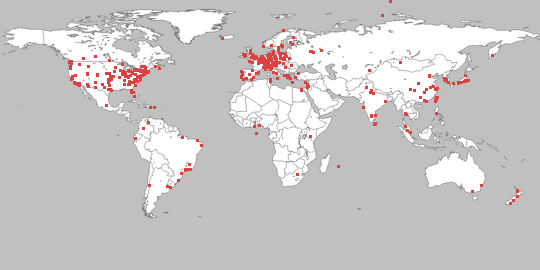
\includegraphics[scale=.6]{world}
\end{figure}

%\noindent\textbf{I am considering the following thesis option(s):}%Remove the comment (percentage) symbol in front of the appropriate category:
%\begin{itemize}
%\item fall one-semester 
%%\item winter one-semester 
%%\item two-semester non-honors
%\item two-semester honors
%\end{itemize}



\bigskip

%\noindent \textbf{Potential Advisor(s) (all relevant fields):} %Write the name of any professor(s) you think you might want to work with on this topic. You may leave this section blank if you don't know. 
%Carl Friedrich Gauss (Mathematics Department)

\bigskip

%\noindent \textbf{Courses I have had which support my thesis proposal:} 
%%List the courses which are relevant; you don't need to list every mathematics course you have ever taken. 
%
%\begin{enumerate}
%\item Real Analysis (Math 301)
%\item Complex Analysis (Math 308)
%\item Abstract Algebra (Math 309)
%\item Topology (Math 313)
%\item Number Theory (Math 365B)
%\end{enumerate} 

\bigskip 

\section*{Proposal}

\bigskip

%This is where you would explain, in detail, what you plan to work on. This should be 1 to 3 pages in length. Here is an example of how you would cite your references in the body of your proposal.






\begin{thebibliography}{99}
% NOTE: change the "9" above to "99" if you have MORE THAN 10 references.

\bibitem{cb} James Ward Brown, Ruel V.~Churchill. \textit{Complex Variables and Applications.} Seventh Edition, McGraw Hill, 2004.   

\bibitem{hadamard} Jacques Hadamard. \textit{Sur la distribution des z\'{e}ros de la fonction $\zeta(s)$ et ses cons\'{e}quences arithm\'{e}tiques}, Bulletin de la Societ\'{e} Math\'{e}matique de France \textbf{14} (1896) pp 199--220.


\end{thebibliography}






%%%%%%%%%%%%%%%%%%%%%%%%%%%%%%%%%%%%%%%%%






\end{document} 
